\documentclass[a4paper,12pt]{article}
\usepackage{template}

\usepackage{booktabs}% for more beautiful hlines


\begin{document}
%QM Postulate und Theoreme
\section{Grundlagen der QM}
\subsection{Wichtige Theoreme f�r die QM}
\begin{tabular}{p{4cm} p{15cm}}
Theorem 1	& Selbstadjungierte, lineare Operatoren haben {\bfseries reelle Eigenwerte}. (Selbstadjungiert: $A_{ij} = A_{ji}^{\ast}$)\\
Theorem 2	& Eigenfunktionen von selbstadjungierten Operatoren sind {\bfseries orthogonal}, wenn sie verschiedene Eigenwerte haben. Eigenfkt. mit gleichen Eigenwerten k�nnen orthogonalisiert werden (z.B. mit Gram-Schmidt).\\
Theorem 3	& Wenn zwei Operatoren $\hat{A}$ und $\hat{B}$ eine gemeinsame Basis von Eigenfkt. $\varphi_i$ haben, dann {\bfseries vertauschen} $\hat{A}$ und $\hat{B}$.\\
Theorem 4	& Wenn zwei Operatoren vertauschen, dann kann man eine vollst�ndige, {\bfseries gemeinsame Basis von Eigenfkt.} der beiden Operatoren ermitteln.
\end{tabular}
\subsection{Postulate der QM}
\begin{tabular}{p{4cm} p{15cm}}
Postulat 1		& Ein abgeschlossenes System wird durch seinen Operator $\hat{H}$ strukturell vollst�ndig charakterisiert.\\
Postulat 2		& $\varphi_n$ sind Eigenfunktionen des Hamilton-Operators $\hat{H}$. $\Psi$ ist ein Element (sog. Zustandsvektor) des Vektorraums, der durch $\varphi_n$ aufgespannt wird, d.h. $\boxed{\Psi = \sum_n c_n \varphi_n}$\\
Skalarprodukt		& $\int \varphi_n^{\ast} \varphi_m d\tau := \int_{-\infty}^{\infty} \cdots \int_{-\infty}^{\infty} \varphi_n^{\ast} (x_1,x_2,...,x_N) \varphi_m(x_1,x_2,...,x_N)dx_1 dx_2 \cdots dx_N$\\
Postulat 3		& Eine Observable entspricht einem selbstadjungiertem, linearem Operator $\hat{A}$. Ein Observable ist genau dann (klassisch) messbar, falls $\boxed{\Psi = \varphi_n$ und $\hat{A}\varphi_n = a_n\varphi_n}$. Ist die Observable nicht messbar, k�nnen nur Aussagen �ber die Erwartungswerte gemacht werden.\\
Postulat 4 (Erwartungswerte)	& Falls $\Psi$ normiert: $\langle \hat{A} \rangle = \int \Psi^{\ast} \hat{A} \Psi d\tau$\\
				& Sonst: $\langle \hat{A} \rangle =\frac{ \int \Psi^{\ast} \hat{A} \Psi d\tau}{ \int \Psi^{\ast} \Psi d\tau}$\\
				& $\boxed{\int \Psi^{\ast} \hat{A} \Psi d\tau = \sum_n |c_n|^2 a_n}\quad |c_n|^2$ ist die WSK, dass die Observable im Zustand $a_n$ ist.\\
QM Messung		& Direkt nach der Messung einer Observablen ist das System in einem Eigenzustand $\varphi_n$ des Messoperators $\hat{A}$. Damit f�hren weitere, identische Messungen am System immer zum selben Ergebnis $a_n$\\
Postulat 5		& \begin{tabular}[t]{ll}
          		  Zeitabh�ngige SG:	& $i\hbar \frac{\partial \Psi}{\partial t} = \hat{H}\Psi$\\
			  Zeitunabh�ngige SG:	& $\hat{H} \Psi = E \Psi$
          		  \end{tabular}\\
Postulat 6		& \begin{tabular}[t]{l}
          		  Zusammenfassung zweier unabh�ngiger Hilbertr�ume $H_1$ und $H_2$\\
			  $H = H_1 \bigotimes H_2\quad \bigotimes \equiv \mathrm{kron}$\\
			  $H = H_1 \bigoplus H_2\quad = H_1 \bigotimes 1 + 1 \bigotimes H_2\quad \text{falls $H_1, H_2$ wechselwirkungsfrei}$
          		  \end{tabular}\\
Separabilit�t der SG (vgl. Bsp. S.3-8)	& \begin{tabular}[t]{l}
			    Falls $H = H_1 \bigoplus H_2$, dann\\
			    $E_{{n_a},{n_b}} = E_{a,{n_a}} + E_{b,{n_b}}$, und\\
			    $\Psi_{{n_a},{n_b}}(\vec{q_i}) = \Psi_{a,{n_a}}(\vec{q_j}) \cdot \Psi_{b,{n_b}}(\vec{q_k})$
			  \end{tabular}\\
Postulat 7		& QM-Systeme mit gleicher Masse, Spin, emag. Momenten sind strikte identisch. Gegen�ber Vertauschung zweier Teilchenkoordinaten ist die Zustandsfkt. entweder symmetrisch (+, Bosonen (ganzzahliger Spin)) oder antisymmetrisch (-, Fermionen (halbganzzahliger Spin, Protonen, Elektronen, etc.))
$\boxed{\Psi(\vec{r_1},m_1,..., \vec{r_k},m_k,..., \vec{r_j},m_j,..., \vec{r_N},m_N) = \pm \Psi(\vec{r_1},m_1,...,\vec{r_j},m_j,...,\vec{r_k},m_k,...,\vec{r_N},m_N)}$\\
\end{tabular}\\
\begin{tabular}{p{4cm} p{15cm}}
Bra-Ket-Notation	& \begin{tabular}[t]{l}
			    $\int \varphi_m^{\ast} \varphi_n d\tau =: \langle \varphi_m | \varphi_n \rangle =: \langle m | n \rangle$\\
			    $\quad\langle m | n \rangle = \delta_{mn}$, falls $\varphi$ orthonormiert.\\
			    $\int \varphi_m^{\ast} \hat{A} \varphi_n d\tau =: \langle \varphi_m | \hat{A}\varphi_n \rangle =: \langle m | A | n \rangle$\\
			    $| n \rangle = \varphi_n \Rightarrow c_n | n \rangle = c_n \varphi_n$\\
			    $\langle m | = \varphi_m^{\ast} \Rightarrow c_m^{\ast} \langle m | = c_m^{\ast} \varphi_m^{\ast}$
			  \end{tabular}\\
Matrixdarstellung	& $A_{nm} = \int \varphi_m^{\ast} \hat{A} \varphi_n d\tau = \langle m | A | n \rangle$\\
AufenthaltsWSK		& $P = \iiint_V |\Psi(x,y,z)|^2 dV\quad V \in \Omega$\\
Normierungsbedinung	& $\iiint_{\Omega} |\Psi(x,y,z)|^2 dV = 1$\\
Akzeptable Wellenfkt.	& \begin{tabular}[t]{ll}\\
                     	  1.	& $\int_{-\infty}^{\infty} \Psi^{\ast} (x) \Psi(x) dx < \infty$\\
			  2.	& $\Psi(x)$ muss eindeutig definiert sein.\\
			  3.	& $\Psi(x) \in C^2$\\
			  4.	& $\Psi(x)$ muss stetig sein.\\
                     	  \end{tabular}\\
Heisenberg'sche Unsch�rferelation	& $\Delta A \Delta B \geq \frac{1}{2} \left| \left\langle \left[ \hat{A}, \hat{B} \right] \right\rangle \right| = \frac{1}{2} \int \Psi^{\ast} \langle \hat{A}, \hat{B} \rangle \Psi d\tau$\\
					& {\itshape Bsp: } $\Delta x \Delta p_x \geq \frac{\hbar}{2}$\\
Ritz'sches Variationsverfahren		& \begin{tabular}[t]{p{14cm}}
                              		  $\frac{\langle \Psi | \hat{H} | \Psi \rangle}{\langle \Psi | \Psi \rangle} \geq E_1$\\
					  $\frac{d}{db} \left( \frac{\langle \Psi | \hat{H} | \Psi \rangle}{\langle \Psi | \Psi \rangle} \right) = 0$, wobei $\Psi$ eine Versuchsfunktion ist mit adjustierbarem Parameter $b$, f�r die gilt: $\lim_{x \to\infty} \Psi(x) = 0$\\
					  Bsp. Versuchsfunktion: $\Psi(x) = e^{-bx^2}$
                              		  \end{tabular}
\end{tabular}
\subsection{Erhaltungss�tze}
\begin{tabular}{p{4cm} p{15cm}}
Erhaltungsgr�sse	& Hat eine Observable $\hat{A}$ einen konstanten Erwartungswert, d.h. $\frac{d}{dt} \langle \hat{A} \rangle = 0$, dann ist sie eine Erhaltungsgr�sse.\\
Zeitabh�ngigkeit von $ \langle \hat{A} \rangle$	& $\frac{d}{dt} \langle \hat{A} \rangle = \frac{i}{\hbar} \left\langle \left[ \hat{H}, \hat{A} \right] \right\rangle$\\
			& $\Rightarrow$ Nur wenn $\hat{A}$ und $\hat{H}$ vertauschen, bleibt $\hat{A}$ �ber die Zeit erhalten.\\
			& Dies gilt unter der Annahme, dass $\frac{d}{dt} \hat{A} = 0$.
\end{tabular}
\begin{tabular}{p{4cm}p{4cm}p{5cm}p{5cm}}
\toprule
Erhaltungsgr�sse	& Bedingung				& Invarianz von $\hat{H}$						& Eigenschaft des freien Raums\\\midrule
\textbf{Impuls} \cr $\hat{\vec{p}} = (\hat{p}_x,\hat{p}_y,\hat{p}_z)$		& $\hat{H}(x_i) = \hat{H}(x_i+a)$						& Beliebige Translation der Koordinaten aller Teilchen des Systems	& Homogenit�t des Potentials ($\frac{dV}{dq} = 0\quad q = (x,y,z)$)\\\midrule
\textbf{Gesamtdrehimpuls} \cr $\hat{\vec{J}} = (\hat{J}_x,\hat{J}_y,\hat{J}_z)$	& $\hat{H}(\theta_i,\phi_i,\chi_i) = \hat{H}(\hat{R}(\theta_i,\phi_i,\chi_i))$	& Beliebige Rotation der Koordinaten aller Teilchen des Systems		& Isotropie des Potentials ($\frac{dV}{d\eta} = 0\quad \eta = (\theta,\phi,\chi)$\\\midrule
\textbf{Parit�t}								& $\hat{H}(q_i) = \hat{H}(-q_i)$						& Inversion der Koordinaten aller Teilchen des Systems		& Inversionssymmetrie\\\bottomrule
\end{tabular}
\subsection{Entartung}
\begin{tabular}{p{4cm}p{15cm}}
Entartung			& Mehrere L�sungen liefern gleichen Eigenwert\\
Entartungsfaktor $g_i$		& Anzahl dieser L�sungen\\
Satz �ber entartete Zust�nde	& Seien $\varphi_1$ und $\varphi_2$ zwei Eigenfkt eines Hamilton-Operator zum selben Eigenwert $E_1 = E_2 = E$. Dann ist eine beliebige Linearkombination $\Psi = c_1\varphi_1 \pm c_2\varphi_2$ auch eine Eigenfkt von $\hat{H}$ zum selben Eigenwert $E$. Dieser Satz gilt allgemein f�r $g$ entartete Zust�nde.
\end{tabular}
%Schr�dingergleichung und lineare Bewegungen
\section{Schr�dingergleichung}
\subsection{Allgemeines}
\begin{tabular}{p{4cm} >{$}p{15cm}<{$}}
``Herleitung'' der SG			& \begin{array}[t]{rl}
						& \Psi(x,t) = \Psi_0 \exp \left( \frac{i}{\hbar} (p_x x-Et) \right) \quad \text{(de Broglie)}\\
				\Rightarrow	& p_x \Psi(x,t) = -i\hbar \frac{\partial}{\partial x} \Psi(x,t)\\
				\Rightarrow	& E \Psi(x,t) = i\hbar \frac{\partial}{\partial t} \Psi(x,t)\\
						& \text{Via Korrespondenzprinzip gilt: $E = \frac{\hat{p}^2}{2m}$}\\
				\Rightarrow	& E \Psi(x,t) = \underbrace{i\hbar \frac{\partial}{\partial t}}_{E} \Psi(x,t) = \underbrace{\frac{-\hbar^2}{2m} \frac{\partial^2}{\partial x^2}}_{H} \Psi(x,t) = \frac{\hat{p}^2}{2m}\Psi(x,t)\\
						& \text{L�sungsansatz (Separation der Variablen): $\Psi(x,t) = \psi(x) \cdot \chi(t)$}\\
				\Leftrightarrow	& \psi(x) i\hbar \frac{\partial \chi(t)}{\partial t} = \chi(t) \cdot \frac{-\hbar^2}{2m} \frac{\partial^2}{\partial x^2} \psi(x)\\
				\Leftrightarrow	& \frac{i \hbar \dot{\chi(t)}}{\chi(t)} = \frac{-\hbar^2}{2m} \frac{\psi''(x)}{\psi(x)} = E\\
				\Rightarrow	& \text{ODE 1: } i\hbar \dot{\chi(t)} = E \chi(t) \Rightarrow \chi(t) = \exp(\frac{-i}{\hbar} Et)\\
						& \text{ODE 2: } \frac{-\hbar^2}{2m} \psi''(x) = E \psi(x)
                 			  \end{array}\\
allgemeine SG				& \hat{H} \Psi = \hat{E} \Psi\\
allg. zeitabh�ngige L�sung		& \psi(\mathbf{r},t) = \psi(\mathbf{r}) e^{-i\frac{E}{\hbar}t} = \psi(\mathbf{r})e^{-i\omega t}\\
Normierungsbedingung			& \int_{-\infty}^{\infty} \Psi^{\ast}(x) \Psi(x) dx = 1 = \int_{-\infty}^{\infty} |\Psi(x)|^2 dx\quad \text{falls $\Psi$ reell}\\
Aufenthalts wahrscheinlichkeitsdichte	& P(x) = \Psi^{\ast}(x)\Psi(x)\\
Delokalisation				& \text{vollst�ndige Delokalisation eines Teilchens, falls $P(x) = konst.$}\\
Heisenberg'sche Unsch�rferelation	& \Delta x \Delta p \geq \tfrac{1}{2} \hbar\\
Kommutator				& \left[\hat{A},\hat{B}\right] \equiv \hat{A}\cdot \hat{B} - \hat{B} \cdot \hat{A}\quad \text{Falls} \left[\hat{A},\hat{B}\right] = 0\Rightarrow \text{A und B gleichzeitig messbar}\\
Operatoren				& \begin{array}[t]{lll}
          				   \hat{r}	& \text{Orts-Operator}	& \hat{r} = (x,y,z)^T \\
					   \hat{p}	& \text{Impuls-Operator}	& \hat{p} = -i\hbar\nabla = -i\hbar (\partial / \partial x, \partial / \partial y , \partial / \partial z)^T\\
					   \hat{H}	& \text{Hamilton-Operator*}	& \hat{H} = \frac{\hat{p}^2}{2m} + E_p(\hat{r}) = -\frac{\hbar^2}{2m}\nabla^2 + E_p(\hat{r})\\
					   \multicolumn{3}{l}{\text{* f�r ein freies Teilchen im Potentialfeld}}
          				  \end{array}\\
\end{tabular}
\subsection{allgemeine L�sung f�r SG mit Potential}
\begin{tabular}{p{4cm} >{$}p{15cm}<{$}}
zeitunabh�ngige Schr�dingergleichung (1-dim)	& -\frac{\hbar^2}{2m}\frac{d^2\psi(x)}{dx^2} + E_{pot}(x)\psi(x) = E\psi(x)\\
L�sung der zeitunabh�ngigen SG		& \begin{array}[t]{ll}
						& \underbrace{\frac{-\hbar^2}{2m}}_{=: -C} \frac{\partial^2}{\partial x^2} \psi(x) = (E-E_{pot}) \psi(x)\\
						& \text{Ansatz: $\psi(x) = e^{ikx}$}\\
				\Rightarrow	&  Ck^2\cdot e^{ikx} = (E-E_{pot}) \cdot e^{ikx}\\
				\Leftrightarrow	& k = \pm\sqrt{\frac{E-E_{pot}}{C}} = \pm\sqrt{\frac{(E-E_{pot})\cdot 2m}{\hbar^2}}\\
				\Rightarrow	& \psi_k(x) = A_k e^{ikx} + B_k e^{-ikx}
                                      	  \end{array}\\
L�sung f�r $E_{pot} = 0$		& \psi_1(x) = Ae^{ikx} + Be^{-ikx}\quad k^2 = \frac{2mE}{\hbar^2}\\
L�sung f�r $E < E_{pot}$		& \psi_2(x) = Ce^{-\alpha x} + De^{\alpha x}\quad \alpha^2 = \frac{2m}{\hbar^2}(E_{pot}-E)\\
L�sung f�r $E > E_{pot}$		& \psi_3(x) = Ee^{i\alpha'x} + Fe^{-i\alpha' x}\quad \alpha'^2 = \frac{2m}{\hbar^2}(E-E_{pot})\\
Stetigkeitsbedingungen			& \psi_i = \psi_j \quad\text{und}\quad \frac{\partial \psi_i}{\partial x} = \frac{\partial \psi_j}{\partial x} \text{ f�r $x=0$}
\end{tabular}
\subsection{Spezifische Probleme}
\subsubsection{Potentialstufe}
\begin{tabular}{p{4cm} >{$}p{15cm}<{$}}
$E_{pot}$	& E_{pot} = \begin{cases} 0 & x < 0 \text{ (Bereich I)}\\ E_0 & x \geq 0 \text{ (Bereich II)}\end{cases}\\\midrule
allg. L�sung ($E < E_{pot}$)	& \begin{array}[t]{l}
      		  \psi_I(x) = Ae^{ikx} + Be^{-ikx}\quad k^2 = \frac{2mE}{\hbar^2}\\
		  \psi_{II}(x) = Ce^{-\alpha x} + De^{\alpha x}\quad \alpha^2 = \frac{2m}{\hbar^2}(E_{pot}-E)
      		  \end{array}\\
Stetigkeitsbedingungen	& \left.\psi_I\right|_{x=0} = \left.\psi_{II}\right|_{x=0} \quad\text{und}\quad \left.\frac{\partial \psi_I}{\partial x}\right|_{x=0} = \left.\frac{\partial \psi_{II}}{\partial x}\right|_{x=0}\\
Randbedingungen	& \lim_{x\to\infty} \psi_{II} < \infty \text{ (vgl. Normierungsbedingung)}\\
spez. L�sung	& \begin{array}[t]{ll}
            	  D = 0 \text{ (aus RB)}	&\\
		  B = \frac{(ik+\alpha)A}{ik-\alpha}	& C = \frac{2ikA}{ik-\alpha}
            	  \end{array}\\\midrule
allg. L�sung ($E > E_{pot}$)	& \begin{array}[t]{l}
      		  \psi_I(x) = Ae^{ikx} + Be^{-ikx}\quad k^2 = \frac{2mE}{\hbar^2}\\
		  \psi_{II}(x) = Ee^{i\alpha'x} + Fe^{-i\alpha' x}\quad \alpha'^2 = \frac{2m}{\hbar^2}(E-E_{pot})
      		  \end{array}\\
spez.L�sung	& \begin{array}[t]{ll}
            	  F = 0 \text{ (aus RB)}	&\\
		  B = \frac{(k-\alpha')A}{k+\alpha'}	& E = \frac{2kA}{k+\alpha'}
            	  \end{array}
\end{tabular}
\subsubsection{Potentialtopf (1D)}
\begin{tabular}{p{4cm} >{$}p{15cm}<{$}}
$E_{pot}$	& E_{pot} = \begin{cases} 0 & 0 < x < a \text{ Bereich I}\\ \infty & \text{ sonst (Bereich II)}\end{cases}\\
allg. L�sung	& \begin{array}[t]{l}
            	  \psi_I(x) = Ae^{ikx} + Be^{-ikx}\quad k^2 = \frac{2mE}{\hbar^2}\\
		  \Leftrightarrow A'\sin(kx) + B'\cos(kx)\\
		  \psi_{II}(x) = 0
            	  \end{array}\\
Randbedigungen	& \psi_I(x=0) = \psi_I(x=a) = 0\\
RB f�r periodische Probleme	& e^{ik\phi} = e^{ik(\phi+2\pi)} \Leftrightarrow 1 = e^{ik2\pi} \Leftrightarrow k = 0,\pm 1,\pm 2 ,... = m_l\\
spez. L�sung	& \psi_I(x) = A' \sin(kx)\quad k = \frac{n\pi}{a} \quad \Rightarrow \lambda = \frac{2\pi}{k} = \frac{2a}{n}\quad n = 1,2,3,...\\
Normierungsbedingung	& A'^2 \int_0^a \sin^2(kx) dx = A'^2 \frac{a}{2} = 1 \Leftrightarrow A = \sqrt{\frac{2}{a}}\\
Energieeigenwert	& E = \frac{\hbar^2 k^2}{2m} = \frac{n^2\pi^2\hbar^2}{2ma^2}
\end{tabular}
\subsubsection{Potentialtopf (3D)}
\begin{tabular}{p{4cm} >{$}p{15cm}<{$}}
SG in 3 Dimensionen			& \psi(x,y,z) = \psi_1(x)\psi_2(y)\psi_3(z)\quad\text{$\psi_{1,2,3}$ sind Wellenfkt. im 1-dim. Kasten}\\
Particle in a cube			& \begin{array}[t]{l}
                 			   \psi(x,y,z) = \sqrt{\frac{8}{a^3}} \sin(\tfrac{n_1\pi}{a} x) \sin(\tfrac{n_2\pi}{a} y) \sin(\tfrac{n_3\pi}{a} z)\\
					   E = \frac{\hbar^2 \pi^2}{2ma^2}(n_1^2+n_2^2+n_3^2)\\
                 			  \end{array}
\end{tabular}
\subsubsection{Der Tunneleffekt}
\begin{tabular}{p{4cm} p{15cm}}
Potentialstufe		& $V(x) = \begin{cases}
              		          0	& x < 0 \quad\text{Bereich A}\\
				  V	& 0 \leq x \leq D \quad\text{Bereich B}\\
				  0	& D < x \quad\text{Bereich C}
              		          \end{cases}$\\
SG			& \begin{tabular}[t]{l}
			    $\hat{H} \Psi_A(x) = -\frac{\hbar^2}{2m} \frac{d^2}{dx^2} \Psi_A(x) = E \Psi_A(x)$\\
			    $\hat{H} \Psi_B(x) = -\frac{\hbar^2}{2m} \frac{d^2}{dx^2} \Psi_B(x) + V \Psi_B(x) = E \Psi_B(x)$\\
			    $\hat{H} \Psi_C(x) = -\frac{\hbar^2}{2m} \frac{d^2}{dx^2} \Psi_C(x) = E \Psi_C(x)$
			  \end{tabular}\\
L�sungen		& \begin{tabular}[t]{ll}
			    $\Psi_A(x) = Ae^{ikx} + Be^{-ikx}$		& $k = \sqrt{\frac{2mE}{\hbar^2}}$\\
			    $\Psi_B(x) = A'e^{ik'x} + B'e^{-ik'x}$	& $k' = \sqrt{\frac{2m(E-V)}{\hbar^2}} = i\kappa$\\
			    $\Psi_C(x) = A''e^{ikx} + B''e^{-ikx}$
        		  \end{tabular}\\
Randbedingungen		& \begin{tabular}[t]{l}
			    $\Psi_A(0) = \Psi_B(0)$\\
			    $\frac{d}{dx} \Psi_A(0) = \frac{d}{dx} \Psi_B(0)$\\
			    $\Psi_B(D) = \Psi_C(D)$\\
			    $\frac{d}{dx} \Psi_B(D) = \frac{d}{dx} \Psi_C(D)$\\
			    $B'' = 0$ (keine reflektierte Komponente rechts der Barriere erlaubt)
			  \end{tabular}
\end{tabular}
Letztlich hat man nur 5 Randbedingungen f�r 6 Unbekannte. Man kann also lediglich die Tunnelwahrscheinlichkeit $P_T = \frac{|A''|^2}{|A|^2}$ angeben, indem man $A''$ durch $A$ ausdr�ckt. $P_T = \frac{4E(V-E)}{4E(V-E) + V^2\sinh^2(\kappa D)}$ Grunds�tzlich wird die Tunnelwahrscheinlichkeit klein f�r breite Barrieren ($D\to\infty$), hohe Barrieren ($V\to\infty$) und grosse Massen $m$

\subsubsection{QM harmonischer Oszillator}
Der QM harmonische Oszillator wird verwendet, um bspw. molekulare Vibrationsbewegungen zu modellieren.
\begin{tabular}{p{4cm} p{2cm}|| p{12cm}}
SG		& \multicolumn{2}{l}{$\hat{H} \Psi = \left( -\frac{\hbar^2}{2m} \frac{d^2}{dx^2} + \frac{1}{2}kx^2 \right) \Psi = E\Psi \qquad(\ast)$}\\
Transformation	& &$\lambda := \frac{2E}{\hbar\omega}\qquad x:= \sqrt{\frac{\hbar}{m\omega}}y \qquad \omega:= \sqrt{\frac{k}{m}}$\\
		& \multicolumn{2}{l}{$(\ast) \Leftrightarrow \left( \frac{d^2}{dy^2} - y^2 \right) \Psi_{\lambda} = -\lambda\Psi_{\lambda}$}\\
Absteigeoperator	& &$a := \frac{1}{\sqrt{2}} \left(y + \frac{d}{dy} \right)$\\
Aufsteigeoperator	& &$a^+ := \frac{1}{\sqrt{2}} \left(y - \frac{d}{dy} \right)$\\
			& &$2aa^+ = -\frac{d^2}{dy^2}+y^2+1$\\
			& &$2a^+a = -\frac{d^2}{dy^2}+y^2-1$\\
			& &$aa^+ = a^+a+1$\\
		& \multicolumn{2}{l}{$(\ast) = -(2aa^+-1)\Psi_{\lambda}$}\\
		& \multicolumn{2}{l}{$(\ast) \Leftrightarrow a^+a\Psi_{\lambda} = \frac{1}{2}(\lambda-1) \Psi_{\lambda}$}\\
		& \multicolumn{2}{l}{$(\ast) \Leftrightarrow aa^+\Psi_{\lambda} = \frac{1}{2}(\lambda+1) \Psi_{\lambda}$}\\
Linksmultiplikation mit $a$	& \multicolumn{2}{l}{$\underbrace{aa^+}_{=a^+a+1}a\Psi_{\lambda} = \frac{1}{2}(\lambda-1)a\Psi_{\lambda}$}\\
		& \multicolumn{2}{l}{$\Leftrightarrow a^+aa\Psi_{\lambda} = \frac{1}{2}(\lambda-3)a\Psi_{\lambda}$}\\
		& \multicolumn{2}{l}{$\Leftrightarrow a^+a \Psi_{\lambda-2} = \frac{1}{2}(\lambda-3) \Psi_{\lambda-2}$}\\
Konsequenz	& \multicolumn{2}{l}{$a\Psi_{\lambda} ~\propto ~\Psi_{\lambda-2}$ und $a^+\Psi_{\lambda} ~\propto ~\Psi_{\lambda+2}$}\\
$\lambda_{min}$	& \multicolumn{2}{l}{$0 = a^+a\Psi_{\lambda_{min}} = \frac{1}{2}(\lambda_{min}-1) \Psi_{\lambda_{min}}$}\\
		& \multicolumn{2}{l}{$\Rightarrow \lambda_{min} = 1$ Mit dem Aufsteigeoperator erh�lt man weitere $\lambda = 1,3,5,7,...$}\\
Eigenwerte	& \multicolumn{2}{l}{$\boldsymbol{E \mu = (\mu + \frac{1}{2})\hbar\omega}, \quad \mu = 0,1,2,...\quad \text{und }\lambda = 2\mu + 1\quad \omega = \sqrt{\frac{k}{m}}$}\\
Eigenfunktionen	& \multicolumn{2}{l}{$\boldsymbol{\Psi_{\mu} = N_{\mu}H_{\mu}(\sqrt{\alpha}x) e^{-\alpha x^2/2 }}\quad \alpha = \frac{\sqrt{mk}}{\hbar}$}
\end{tabular}
\subsubsection{3D QM harm. Osz.}
\begin{tabular}{p{4cm} p{15cm}}
Eigenwerte	& $E_n = (n_x + n_y + n_z + \frac{3}{2})\hbar\omega$\\
Eigenfunktionen	& $\Psi_n = \Psi_{n_x} \cdot \Psi_{n_y} \cdot \Psi_{n_z}$
\end{tabular}
\subsection{Wellengruppen}
\begin{tabular}{p{4cm} p{15cm}}
L�sungen der zeitabh. SG	& $\Psi_n(q_i,t) = \varphi_n(q_i)e^{-iE_nt/\hbar}$\\
WSKDichte			& Die WSKdichte $|\Psi_n(q_i,t)|^2$ ist zeitunabh�ngig, da\\
				& $|\Psi_n(q_i,t)|^2 = \varphi_n^{\ast}(q_i)e^{iE_nt/\hbar} \cdot \varphi_n(q_i)e^{-iE_nt/\hbar} = |\varphi_n(q_i)|^2$\\
allg. L�sung der SG		& $\Psi(q_i,t) = \sum_n c_n \varphi_n(q_i)e^{-iE_nt/\hbar}$
\end{tabular}
%QM Drehimpulse
\section{QM Drehimpulse}
\begin{tabular}{ll}
Symbol		& Drehimpuls\\\hline
$\vec{l}$	& Bahndrehimpuls eines Elektrons\\
$\vec{s}$	& Spin eines Elektrons\\
$\vec{j}$	& Gesamtdrehimpuls eines Elektrons\\
$\vec{L}$	& Gesamtbahndrehimpuls eines Atoms oder Molek�ls\\
$\vec{S}$	& Gesamtelektronenspin eines Atoms oder Molek�ls\\
$\vec{J}$	& Gesamtdrehimpuls ohne Kernspin\\
$\vec{I_i}$	& Kernspin des i-ten Kerns eines Molek�ls\\
$\vec{F}$	& Gesamtdrehimpuls
\end{tabular}
\subsection{Quantenzahlen}
\begin{tabular}[t]{p{3cm}lll|lll}
			& \multicolumn{3}{l}{klassisch, via Korrespondenzprinzip}	& \multicolumn{3}{l}{QM, allgemein via Kommutatoren}\\
Hauptquantenzahl	& n & 1,2,3,... & unlimitiert\\
			&   & K,L,M,... &\\
Drehimpuls- quantenzahl	& l & 0,1,2,... n-1 & n m�gliche Werte			& J & 0, $\tfrac{1}{2}$,1, $\tfrac{3}{2}$,2,...\\
			&   & s,p,d,f,..    &\\
magnetische Quantenzahl	& $m_l$ & -l, l+1,..., l-1, l& 2l+1 m�gliche Werte	& M & -J,-J+1,...,J-1,J	& 2J+1 m�gliche Werte\\
\end{tabular}
\subsection{Bahndrehimpuls}
\begin{tabular}{p{4cm} p{15cm}}
Klassische Definition		& $\vec{l} = \vec{r} \times \vec{p}$\\
				& $|\vec{l}| = |\vec{r}||\vec{p}| \sin\alpha$\\
QM Definition			& $\hat{\vec{l}} = -i\hbar
					\begin{pmatrix}
					y\frac{\partial}{\partial z} - z\frac{\partial}{\partial y}\\ 
					z\frac{\partial}{\partial x} - x\frac{\partial}{\partial z}\\ 
					x\frac{\partial}{\partial y} - y\frac{\partial}{\partial x}
					\end{pmatrix}$\\
				& $|\vec{l}|^2 = \hat{l}^2 = \hat{l}_x^2 + \hat{l}_y^2 + \hat{l}_z^2$\\
Vertauschungsrelationen		& $[\hat{l}_x, \hat{l}_y] = i\hbar \hat{l}_z, \quad [\hat{l}_x, \hat{l}_z] = i\hbar \hat{l}_y, \quad[\hat{l}_y, \hat{l}_z] = i\hbar \hat{l}_x$\\
				& $[\hat{l}^2, \hat{l}_x] = 0, \quad [\hat{l}^2, \hat{l}_y] = 0, \quad [\hat{l}^2, \hat{l}_z] = 0$\\
				& Gem�ss Thm. 4 haben also $\hat{l}^2$ und $\hat{l}_z$ eine gemeinsame Basis von Eigenfunktionen:\\
Gel�ste Eigenwertgleichungen	& \begin{tabular}[t]{|lll|}
						  \hline
						  $\hat{l}^2 Y(\theta,\phi) = \hbar^2 l(l+1)  Y(\theta,\phi)$	& $l = 0,1,2,...$		& $l$: Bahndrehimpulsquantenzahl\\
                                             	  $\hat{l}_z Y(\theta,\phi) = \hbar m Y(\theta,\phi)$		& $m = -l,-l+1,...,l-1,l$	& $m$: magnetische Quantenzahl\\\hline
                                             	  \end{tabular}\\
Bra-Ket Notation		& $Y_{l,m} = |l,m \rangle$\\
Unbestimmtheitsrelation		& $\Delta l_x \Delta l_y \geq \frac{1}{2} |\langle [\hat{l}_x, \hat{l}_y] \rangle | = \frac{1}{2} \hbar | \langle \hat{l}_z \rangle |$\\
Spherical Harmonics		& $Y_{l,m} (\theta,\phi) = N_{l,m} P_l^{|m|} (\cos \theta) e^{im\phi}, \text{wobei } N_{l,m} = \sqrt{\frac{(2l+1)(l-|m|)!}{4\pi(l+|m|)!}}$\\
\textbf{Parit�t von $Y_{l,m}$}	& $\boxed{\text{Parit�t}(Y_{l,m}) = (-1)^l}$\\
Legendre-Polynome		& \begin{tabular}[t]{l}
				    $P_n^m(z) \equiv (1-z^2)^{m/2} \frac{d^m}{dz^m}P_n(z)$\\
				    $P_n(z) = \frac{ 1}{2^n n!}\frac{d^n}{dz^n}(z^2-1)^n$\\
				    $P_0^0 = 1, ~~ P_1^0 = z, ~~ P_1^1 = (1-z^2)^{1/2}$\\
				    $P_2^0 = \frac{1}{2} (3z^2-1), ~~ P_2^1 = 3(1-z^2)^{1/2}\cdot z, ~~ P_2^2 = 3(1-z^2)$
				  \end{tabular}\\
\end{tabular}
\subsection{Allgemeine Drehimpulse}
Allg. Drehimpulse $J$ werden rein quantenmechanisch mit Vertauschungsrelationen definiert, es existiert f�r sie kein klassisches Analogon. Erkl�rt werden kann damit der Spin.\\
\begin{tabular}{p{4cm} p{15cm}}
Vertauschungsrelationen		& $[\hat{J}_x, \hat{J}_y] = i\hbar \hat{J}_z, \quad [\hat{J}_x, \hat{J}_z] = i\hbar \hat{J}_y, \quad[\hat{J}_y, \hat{J}_z] = i\hbar \hat{J}_x$\\
				& $[\hat{J}^2, \hat{J}_x] = 0, \quad [\hat{J}^2, \hat{J}_y] = 0, \quad [\hat{J}^2, \hat{J}_z] = 0$\\
Gel�ste Eigenwertgleichungen	& \begin{tabular}[t]{|lll|}
				    \hline
				    $\hat{J}^2 \Psi = \hbar^2 J(J+1)  \Psi$	& $J = 0,\frac{1}{2},1,\frac{3}{2},...$	& $J$: Drehimpulsquantenzahl\\
                                    $\hat{J}_z \Psi = \hbar M \Psi$		& $M = -J, -J+1,...,J-1,J$		& $M$: magnetische Quantenzahl\\\hline
                                  \end{tabular}\\
Bra-Ket Notation		& $\Psi_{J,M} = |J,M \rangle$\\
Orientierung von Drehimpulsvektoren& \begin{tabular}[t]{lll}
				    $|\vec{J}| = \hbar \sqrt{J(J+1)}$	& L�nge		& Entartung: $2J+1$\\
				    $J_z = \hbar M$			& z-Komponente	& Entartung: 1
				  \end{tabular}
\end{tabular}
\subsection{Matrixdarstellung von Drehimpulsoperatoren}
\begin{tabular}{p{4cm} p{15cm}}
Matrixdarstellung eines Operators	& $A_{nm} = \int \Psi_n^{\ast} \hat{A} \Psi_m = \langle n | \hat{A} | m \rangle$ Achtung! Nicht mit Erwartungswert verwechseln!\\
Aufsteigeoperator			& $\hat{J}_+ = \hat{J}_x + i\hat{J}_y$\\
Absteigeoperator			& $\hat{J}_- = \hat{J}_x - i\hat{J}_y$\\
					& $\hat{J}_x = \frac{\hat{J}_+ + \hat{J}_-}{2}$\\
					& $\hat{J}_y = \frac{\hat{J}_+ - \hat{J}_-}{2i}$\\
$\hat{J}_z$				& $\langle J',M' | \hat{J}_z | J,M \rangle = \hbar M \langle J',M' | J,M \rangle = \hbar M \delta_{J',J} \delta_{M',M}$\\
$\hat{J}^2$				& $\langle J',M' | \hat{J}^2 | J,M \rangle = \hbar^2 J(J+1) \langle J',M' | J,M \rangle = \hbar M \delta_{J',J} \delta_{M',M}$\\
$\hat{J}_+$				& $\langle J',M' | \hat{J}_+ | J,M \rangle = \hbar \sqrt{J(J+1)-M(M+1)} \delta_{J',J} \delta_{M',M+1}$\\
$\hat{J}_-$				& $\langle J',M' | \hat{J}_- | J,M \rangle = \hbar \sqrt{J(J+1)-M(M-1)} \delta_{J',J} \delta_{M',M-1}$\\
\end{tabular}
\subsubsection{Pauli-Matrizen}
Beispiel f�r eine Matrixdarstellung f�r $J = \frac{1}{2} \Rightarrow M = \pm \frac{1}{2}$. (Spin 1/2 Teilchen)\\
Es gibt also nur zwei Eigenfunktionen: $|\tfrac{1}{2}, \tfrac{1}{2} \rangle = : |\alpha \rangle$ und $|\tfrac{1}{2}, -\tfrac{1}{2} \rangle =: |\beta\rangle$\\
\begin{tabular}{p{4cm} p{15cm}}
$\hat{J}_z$	& $\hat{J}_z = \begin{bmatrix} \langle \alpha | \hat{J}_z | \alpha \rangle 	& \langle \alpha | \hat{J}_z | \beta \rangle \\
				\langle \beta | \hat{J}_z | \alpha \rangle 			& \langle \beta | \hat{J}_z | \beta \rangle \end{bmatrix}
			      = \frac{\hbar}{2} \begin{bmatrix}1 & 0\\0 & -1\end{bmatrix} = \frac{\hbar}{2} \sigma_z$\\
$\hat{J}^2$	& $\hat{J}^2 = \hbar^2 \begin{bmatrix} \tfrac{3}{4} & 0 \\ 0 & \tfrac{3}{4} \end{bmatrix} = \frac{3\hbar^2}{4} \mathbb{I}_2$\\
$\hat{J}_x$	& $\hat{J}_x = \frac{\hat{J}_+ + \hat{J}_-}{2} = \frac{\hbar}{2} \begin{bmatrix}0 & 1 \\ 1 & 0\end{bmatrix} = \frac{\hbar}{2} \sigma_x$\\
$\hat{J}_y$	& $\hat{J}_y = \frac{\hat{J}_+ + \hat{J}_-}{2i} = \frac{\hbar}{2} \begin{bmatrix}0 & -i \\ i & 0\end{bmatrix} = \frac{\hbar}{2} \sigma_y$\\
\end{tabular}





%Rotation starrer Molek�le
\section{Rotation starrer Molek�le}
\begin{tabular}{p{4cm} p{15cm}}
Tr�gheitsmoment			& $I = \sum_i m_ir_i^2$\\
Tr�gheitsmoment f�r 2-atomiges Molek�l	& $I = \mu R^2 \quad \mu = \frac{m_1m_2}{m_1+m_2}\quad R:$ Molek�labstand\\
Drehimpulse			& \begin{tabular}{ll}
				  in raumfesten Koordinaten	& $\hat{J}_x, \hat{J}_y, \hat{J}_z$\\
				  in k�rperfesten Koordinaten	& $\hat{J}_X, \hat{J}_Y, \hat{J}_Z$
           			  \end{tabular}\\
Klassische Definition	& \begin{tabular}{l}
				$E_{rot} = \frac{1}{2} I \vec{\omega}^2 = \frac{\vec{J}^2}{2I}$\\
				$\quad I$: Tr�gheitsmoment um Drehachse $\omega$\\
				$\quad J = I\vec\omega$: Drehimpulsvektor des K�rpers.
			\end{tabular}\\
Andere Schreibweise		& $E_{rot} = \frac{1}{2} \vec\omega^T \boldsymbol{I} \vec\omega = \frac{1}{2} \left( \frac{J_X^2}{I_X} + \frac{J_Y^2}{I_Y} + \frac{J_Z^2}{I_Z} \right)$\\
QM Definition		& \begin{tabular}{rcl}
			    $\hat{H}_{rot} \Psi_{rot}$ & = & $E_{rot} \Psi_{rot}$, wobei\\
			    $\hat{H}_{rot}$		&= & $\frac{1}{2} \left( \frac{J_X^2}{I_X} + \frac{J_Y^2}{I_Y} + \frac{J_Z^2}{I_Z} \right)$
			  \end{tabular}\\
Anomale Vertauschungsrelationen	& $[\hat{J}_x, \hat{J}_y] = -i\hbar \hat{J}_z, \quad [\hat{J}_x, \hat{J}_z] = -i\hbar \hat{J}_y, \quad[\hat{J}_y, \hat{J}_z] = -i\hbar \hat{J}_x$\\
				& $[\hat{J}^2, \hat{J}_x] = 0, \quad [\hat{J}^2, \hat{J}_y] = 0, \quad [\hat{J}^2, \hat{J}_z] = 0$\\
Gel�ste Eigenwertgleichungen	& \begin{tabular}[t]{|lll|}
				    \hline
				    $\hat{J}^2 \Psi = \hbar^2 J(J+1)  \Psi$	& $J = 0,\frac{1}{2},2,\frac{3}{2},...$	& $J$: Drehimpulsquantenzahl\\
                                    $\hat{J}_z \Psi = \hbar M \Psi$		& $M = -J, -J+1,...,J-1,J$		& $M$: magnetische Quantenzahl\\
                                    $\hat{J}_Z \Psi = \hbar K \Psi$		& $K = -J, -J+1,...,J-1,J$		&\\\hline
                                  \end{tabular}\\
Bra-Ket Notation		& $\Psi_{rot; J,K,M} = |J,K,M \rangle$\\
Rotationskonstanten		& \begin{tabular}[t]{l}
				    $\tilde{A} = \frac{\hbar}{4\pi c I_a} = \frac{A}{c}$\\
				    $\tilde{B} = \frac{\hbar}{4\pi c I_a} = \frac{B}{c}$\\
				    $\tilde{C} = \frac{\hbar}{4\pi c I_a} = \frac{C}{c}$\\
				    wobei $\tilde{X}$ in Wellenzahleinheiten, $X$ in Frequenzeinheiten
				  \end{tabular}
\end{tabular}
\subsection{Beispiel 1: sph�rischer Kreisel}
\begin{tabular}{p{4cm} p{15cm}}
Tr�gheitsmomente	& $I_X = I_Y = I_Z = I$\\
Hamilton-Operator	& $\hat{H}_{rot} = \frac{1}{2I} \left( \hat{J}_X^2 + \hat{J}_Y^2 + \hat{J}_Z^2 \right) = \frac{1}{2I} \hat{J}^2$\\
Energieeigenwerte	& $E_{J,K,M} = E_J = \frac{\hbar^2}{2I} J(J+1) = hc\tilde{B} J(J+1)$\\
Entartung		& $g_J = (2J+1)^2$ (volle Entartung durch M und K)\\
\end{tabular}
\subsection{Beispiel 2: symmetrischer Kreisel}
\begin{tabular}{p{4cm} p{15cm}}
Tr�gheitsmomente	& $I_X = I_Y \neq I_Z$\\
Hamilton-Operator	& $\hat{H}_{rot} = \frac{\hat{J}_X^2 + \hat{J}_Y^2}{2I_X} + \frac{\hat{J}_Z^2}{2I_Z} =  \frac{\hat{J}^2 - \hat{J}_Z^2}{2I_X} + \frac{\hat{J}_Z^2}{2I_Z}$\\
Energieeigenwerte	& \begin{tabular}[t]{ll}
			    $E_{J,K,M} = E_{J,K} = \frac{\hbar^2}{2I_X} J(J+1) + \left(\frac{\hbar^2}{2I_Z} - \frac{\hbar^2}{2I_X}\right)K^2$\\
			    $ = hc\tilde{B} J(J+1) + hc (\tilde{A} - \tilde{B})K^2$	& (spindelf�rmiger Kreisel)\\
			    $ = hc\tilde{B} J(J+1) + hc (\tilde{C} - \tilde{B})K^2$	& (tellerf�rmiger Kreisel)\\
			  \end{tabular}\\
Entartung		& $g_{J,K} = \begin{cases}
         		             (2J+1) \cdot 2 & K \neq 0\\
				     2J+1	    & K = 0
         		             \end{cases}$
\end{tabular}
\subsection{Beispiel 3: zweiatomige Molek�le}
Spezialfall von symmetrischem Kreisel mit $I_Z = 0 \Rightarrow K = 0$




%Drehimpulssysteme in Magnetfeldern, Addition von Drehimpulsen
\section{Drehimpulssysteme in Magnetfelder}
\subsection{Klassische Behandlung}
\begin{tabular}{p{4cm} p{15cm}}
magnetisches Moment	& $\vec\mu = IA\vec n\quad $I = Stromst�rke, A = Fl�che, n = Normalenvektor auf A\\
externes Magnetfeld	& $\vec B$\\
potentielle Energie	& $E_{pot} = -|\mu||B| \cos \theta = -\vec\mu \cdot \vec B$\\
magnetisches Moment	& $\vec\mu = \gamma_l \vec l \quad \gamma_l = -\frac{e}{2m_e} = g_l \frac{\mu_B}{\hbar}$\\
			& $\vec l$: Bahndrehimpuls, $\mu_B$: Bohr'sches Magneton, $g_l$: Proportionalit�tsfaktor\\
			& $\Rightarrow E_{pot} = -\vec\mu \cdot \vec B = -\gamma_l \vec l \cdot \vec B = -\gamma_l (l_xB_x + l_yB_y + l_zB_z)$
\end{tabular}
\subsection{QM Behandlung (Korrespondenzprinzip)}
\begin{tabular}{p{4cm} p{15cm}}
Hamilton-Operator (Kern-Zeeman)	& $\hat{H}_N = -\gamma_N \left( \hat{I}_xB_x + \hat{I}_yB_y + \hat{I}_zB_z \right)\quad$ wobei $\hat{I}$ ein Drehimpulsoperator ist (vgl.Pauli-Matrix)
\end{tabular}

\section{Addition von Drehimpulsen}
Sei $\hat{\vec J} = \hat{\vec{j}}_1 + \hat{\vec{j}}_2$ der resultierende Drehimpuls.\\
\begin{tabular}{p{4cm} p{15cm}}
Zugeh�rige Quantenzahlen	& \begin{tabular}[t]{l}
                        	  $\hat{\vec{j}}_1: |j_1,m_1\rangle$\\
				  $\hat{\vec{j}}_2: |j_2,m_2\rangle$\\
				  $\hat{\vec{J}}: |J,M\rangle$
                        	  \end{tabular}\\
gekoppelte Darstellung (gD)	& $|j_1,m_1,J,M \rangle$: In der gekoppelten Darstellung setzt man die Quantenzahlen $J$ und $M$ fest. \\
ungekoppelte Darstellung (uD)	& $|j_1,m_1,j_2,m_2 \rangle$: In der ungekoppelten Darstellung setzt man $j_1,m_1,j_2,m_2$ fest.\\
\multicolumn{2}{l}{gD und uD spannen denselben Vektorraum auf. Sie sind lediglich verschiedene S�tze von Basisfunktionen.}\\
Betrag und z-Komponente (gD)	& \begin{tabular}[t]{lcl}
				    $|\vec{J}| = \hbar \sqrt{J(J+1)}$	& $\Rightarrow $	& $|\vec{J}| = |\vec{j_1} + \vec{j_2}| = ??$\\
				    $J_z = \hbar M$			& $\Rightarrow $	& $J_z = j_{1,z} + j_{2,z} = \hbar(m_1 + m_2)$
				  \end{tabular}\\
\multicolumn{2}{l}{$M$ ist immer gleich $m_1 + m_2$. Weil $|M| \leq |J|$ sein muss, k�nnen wir die m�glichen Werte f�r $J$ aus $M$ ableiten.}\\
Resultierende Quantenzahlen (gD)	& \begin{tabular}[t]{|l|}
				  \hline
                           	  $J = j_1 + j_2, j_1 + j_2 - 1,..., |j_1-j_2|$ \\
				  $M = m_1 + m_2$\\\hline	
                           	  \end{tabular}\\
Bra-Ket Notation (gD)		& $|j_1,j_2,J,M\rangle$\\
Anzahl Basisfunktionen (gD,uD)	& $\underbrace{(j_1+j_2)}_{\text{\# J-Werte}} \cdot \underbrace{(2(j_1+j_2) + 1)}_{\text{\# M-Werte pro J-Wert}}$\\
Umrechnung gD - uD		& \begin{tabular}[t]{lcl}
                        	  $|j_1,m_1,j_2,m_2\rangle$	& = &	$|j_1,m_1\rangle |j_2,m_2\rangle$\\
				  $|j_1,j_2,J,M \rangle$	& = &	$\sum_{j_1,m_1,j_2,m_2} \underbrace{c(j_1,m_1,j_2,m_2,J,M)}_{\text{Clebsch-Gordan Koeffizienten}}|j_1,m_1,j_2,m_2\rangle$
                        	  \end{tabular}
\end{tabular}





%Atome
\section{Atome}
\subsection{Wasserstoffatom}
\begin{tabular}{p{4cm} p{15cm}}
Schr�dingergleichung	& $\hat{H} = \underbrace{-\frac{\hbar^2}{2m_K} \nabla^2_K}_{E_{kin}\text{ des Kerns}} \underbrace{ -\frac{\hbar^2}{2m_e} \nabla^2_e}_{E_{kin}\text{ des Elektrons}} - \frac{Ze^2}{4\pi\epsilon_0 r} +$ andere Terme\\
Umformung der SG (vgl. Kap. 4.5)	& $\hat{H} = \underbrace{-\frac{\hbar^2}{2M}\nabla^2_{SP}}_{\text{Schwerpunktbew.}} \underbrace{-\frac{\hbar^2}{2\mu}\nabla^2_r-\frac{Ze^s}{4\pi\epsilon_0 r}}_{\text{interne Bewegung}}$\\
vereinfachte SG		& \begin{tabular}[t]{l}
               		  $\hat{H}\Psi = \left( -\frac{\hbar^2}{2\mu} \nabla^2_r - \frac{Ze^2}{4\pi\epsilon_0 r} \right) \Psi = E\Psi$ (QM Coulomb-Potential)\\
			  $\mu = \frac{m_e \cdot m_K}{m_e + m_K} \approx m_e$\\
			  $M = m_e + m_K$\\
			  $Z =$ Kernladungszahl
               		  \end{tabular}\\
Ansatz f�r Eigenfkt.	& $\Psi(r,\theta,\phi) = R(r) \cdot Y_{lm}(\theta,\phi)$\\
L�sungen		& \begin{tabular}[t]{lcll}
			  $R_{n,l}(r)$	& = & $N_{n,l} \exp \left\lbrace -\frac{Zr}{na} \right\rbrace \left( \frac{2Zr}{na} \right)^l L^{2l+1}_{n-l-1}\left( \frac{2Zr}{na} \right)$	&$n = 1,2,...$\\
			  \multicolumn{4}{l}{$a = \frac{m_e}{\mu}a_0;\quad a_0 = \frac{4\pi \epsilon_0 \hbar^2}{m_e e^2} = 0.0529 nm$}\\
        		  $Y_{lm}$	& = & Eigenfkt. des Drehimpulsoperators		& $l = 1,...,(n-1)$\\
					&	&					& $m = -l,-l+1,...l$\\
			  \multicolumn{4}{l}{Superpositionen sind nat�rlich auch wieder L�sungen!}
        		  \end{tabular}\\
Energieeigenwerte	& \begin{tabular}[t]{l}
                 	  $E_{n,l,m} = E_n = -\frac{hcRZ^2}{n^2} = -13.606eV \frac{Z^2}{n^2}$\\
			  $c =$ Lichtgeschwindigkeit; $R = \frac{\mu e^4}{8\epsilon_0^2h^3c}$
                 	  \end{tabular}\\
Entartung		& $g = \sum_{l=0}^{n-1} (2l+1) = n^2$ (Pro $l$ gibt es $2l+1$ $m$)\\
radiale WSKDichte	& \begin{tabular}[t]{ll}
                 	  WSKDichte		&$p_{n,l}(r) dr = |R_{n,l}(r)^2| r^2 dr$\\
			  Radius des Maximums	& $\arg\max_r p_{n,l}(r) = r_{pmax} = \frac{n^2}{Z}a$ (Bohr'scher Atomradius)\\
			  Mittlerer Radius	& $\frac{a}{2Z} \left(3n^2-l(l+1) \right)$
                 	  \end{tabular}\\
Auswahlregeln (Atom�berg�nge) 	& \begin{tabular}[t]{l}
             		  Emission und Absorption von Photonen:\\
			  $\Delta l = l_f - l_i = \pm 1$\\
			  $\Delta j = j_f - j_i = 0, \pm 1\quad j_i = 0 \Rightarrow j_f \neq 0$\\
			  Nur diese �berg�nge k�nnen im Spektrum erscheinen.
             		  \end{tabular}\\
\end{tabular}
\subsection{Mehrelektronenatome}
\begin{tabular}{p{4cm} p{15cm}}
Ein Protonen, zwei Elektron System	& $E_{pot} = -\frac{Ze^2}{4\pi\epsilon_0 r_1} -\frac{Ze^2}{4\pi\epsilon_0 r_2} + \underbrace{\frac{e^2}{4\pi\epsilon_0 r_{12}}}_{Elektron-Elektron-Abstossung}$\\
Permutationsoperator	& \begin{tabular}[t]{l}
                    	  $\hat{P}_{12} \Psi_A(1)\Psi_B(2) = \Psi_A(2)\Psi_B(1)$\\
			  $\left[ \hat{P}, \hat{H} \right] = 0$
                    	  \end{tabular}\\
Satz			& Sei $f(\vec{q}_1, ... , \vec{q}_i, \vec{q}_j,..., \vec{q}_n)$ eine beliebige Funktion. Dann sind die Funktionen $\Psi^{\pm}(\vec{q}_1,...,\vec{q}_n) = f(\vec{q}_1, ... , \vec{q}_i, \vec{q}_j,..., \vec{q}_n) \pm f(\vec{q}_1, ... , \vec{q}_j, \vec{q}_i,..., \vec{q}_n)$ Eigenfunktionen von $\hat{P}_{ij}$ zu den Eigenwerten $\pm 1$\\
Verallgemeinertes Pauli-Prinzip	& \begin{itemize}
                               	  	\item Eigenfkt von $\hat{H}$ sind entweder symmetrisch oder antisymmetrisch bzgl. der Permutation zweier identischer Teilchen (iT).
					\item Eigenfkt m�ssen symmetrisch sein bzgl. einer Permutation zweier iT mit ganzzahligem Spin. (Bosonen)
					\item Eigenfkt m�ssen antisymmetrisch sein bzgl. einer Permutation zweier iT mit halbganzzahligem Spin. (Fermionen, z.B.Elektronen)
                               	  \end{itemize}\\
\multicolumn{2}{p{19cm}}{$\Rightarrow$ Weil Elektronen Fermionen sind, m�ssen die Gesamtwellenfkt. von Mehrelektronenatomen antisymmetrisch sein!}\\
Bahnwellenfunktion Atom			& $\Psi_{Atom}(2,1) =  \Psi_a(2)\Psi_b(1) \pm \Psi_a(1) \Psi_b(2) = \pm \Psi_{Atom}(1,2)\quad$ a,b: Zust�nde; 1,2: Elektronen\\
symmetrische Bahnwellenfunktion		& \begin{tabular}[t]{l}
                               		  	$\Psi_S(1,2) = \Psi_S(2,1)\quad \lim_{a\to b} \Psi_S > 0$\\
						$\Rightarrow$ Elektronen k�nnen einander nahe kommen $\Rightarrow$ Hohe mittlere Abstossungsenergie
                               		  \end{tabular}\\
antisymmetrische Bahnwellenfkt.		& \begin{tabular}[t]{l}
                               		  $\Psi_A(1,2) = -\Psi_A(2,1)\quad \lim_{a\to b} \Psi_A = 0$\\
					  $\Rightarrow$ Elektronen sind einander nie nahe $\Rightarrow$ Niedrige mittlere Abstossungsenergie
                               		  \end{tabular}\\
gleiche Zust�nde		& Die Zust�nde $a,b,c,...$ entsprechen Quantenzust�nden $n,l,m_l$. Sind zwei Elektronen im gleichen Zustand, so ist die antisymmetrische Bahnwellenfkt. $\Psi_A(1,2) = \Psi_a(2)\Psi_a(1) - \Psi_a(1)\Psi_a(2) = 0$ und somit nicht erlaubt.\\
Spins				& Die Spins der beiden Elektronen betragen jeweils $\frac{1}{2}$. Je nach Orientation (parallel, antiparallel) k�nnen sie sich zu 0 oder 1 addieren\\
Spinwellenfkt			& $|\alpha \rangle$ bezeichne die Spinwellenfkt bzgl. $m_s = \tfrac{1}{2}$, $|\beta \rangle$ diejenige bzgl. $m_s = -\tfrac{1}{2}$\\
Gesamtspin $S=0$ (Singulett)	& $\chi_A = \alpha(1)\beta(2)-\alpha(2)\beta(1)\quad M_S = 0$ antisymmetrische Spin-Wellenfkt\\
Gesamtspin $S=1$ (Triplett)	& \begin{tabular}[t]{ll}
                           	   $\chi_S = \alpha(1)\alpha(2)$	& $M_S = 1$\\
				   $\chi_S = \alpha(1)\beta(2) + \alpha(2)\beta(1)$	& $M_S = 0$\\
				   $\chi_S = \beta(1)\beta(2)$	& $M_S = -1$
                           	  \end{tabular} symmetrische Spin-Wellenfkt.\\
				& 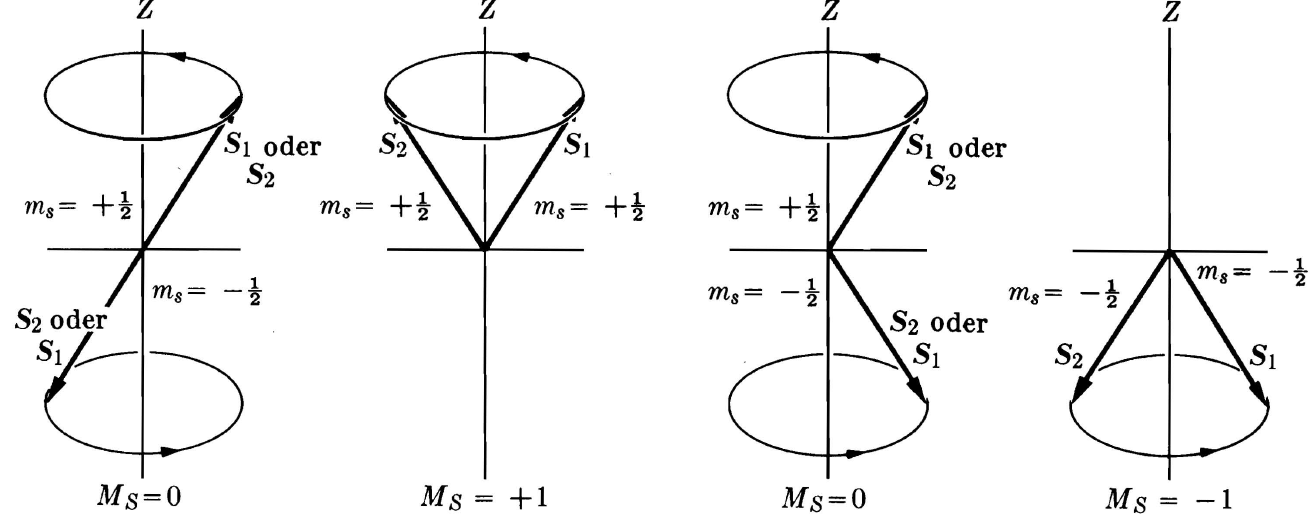
\includegraphics[width = 14cm]{qm_spin.png}\\
\end{tabular}\\\newpage
\begin{tabular}{p{4cm}p{15cm}}
Gesamtwellenfunktion		& \begin{tabular}[t]{p{14cm}}
                    		  $\Psi_{Gesamt} = $ Bahnwellenfkt $\cdot$ Spinwellenfkt = f�r Fermionen immer ANTIsymmetrisch, f�r Bosonen immer symmetrisch. Weil Elektronen Fermionen sind, m�ssen Gesamtwellenfkt. von Atomen immer antisymmetrisch sein.\\
				  Singuletts: symmetrische Bahnwfkt $\cdot$ antisymmetrische Spinwfkt.\\
				  Tripletts: antisymmetrische Bahnwfkt $\cdot$ symmetrische Spinwfkt.\\
				  $\Rightarrow$ Tripletts haben eine tiefere Energie als der Singulett-Zustand (wegen Bahnwfkt, siehe oben)
                    		  \end{tabular}\\

antisymmetrische Gesamtwfkt (Slater-Determinante)	&
				  $\Psi_{abc...} = \frac{1}{\sqrt{N!}} \begin{vmatrix} \varphi_a(1)	& \varphi_b(1)	& \varphi_c(1)	& \dotsc\\
										       \varphi_a(2)	& \varphi_b(2)	& \varphi_c(2)	& \dotsc\\
										       \varphi_a(3)	& \dotsc	& \dotsc	& \dotsc\\
										       \dotsc		& \dotsc	& \dotsc	& \dotsc\\
                   		                                       \end{vmatrix}$\\
Bsp. f�r $1s^2$-Zustand		& \begin{tabular}[t]{l}
				  $\Psi_{\alpha\beta}(1,2) = \frac{1}{\sqrt{2}} \begin{vmatrix} |1s(\vec{r}_1)\alpha(1)\rangle	& |1s(\vec{r}_2)\beta(1)\rangle\\
											        |1s(\vec{r}_1)\alpha(2)\rangle	& |1s(\vec{r}_2)\beta(2)\rangle
                       		                                                \end{vmatrix}$\\
				  $= \frac{1}{\sqrt{2}} (|1s(\vec{r}_1)\alpha(1)\rangle |1s(\vec{r}_2)\beta(2)\rangle - |1s(\vec{r}_1)\alpha(2)\rangle |1s(\vec{r}_2)\beta(1)\rangle)$\\
				  $= \frac{1}{\sqrt{2}} \underbrace{|1s(\vec{r}_1\rangle |1s(\vec{r}_2)\rangle}_{Raumteil} \underbrace{(\alpha(1)\beta(2) - \alpha(2)\beta(1))}_{Spinteil}$
				  \end{tabular}\\
Ausschliessungsprinzip		& Jeder Quantenzustand $(n,l,m_l,m_s)$ kann h�chstens von einem Elektron (allg. Fermionen) eingenommen werden. Die Anzahl Zust�nde ist somit beschr�nkt durch die Abh�ngigkeiten der Quantenzahlen.\\
Besetzungszahl (max. \# $e^-$ f�r ein Atom)	& 2(2l+1)
\end{tabular}
\subsection{Konfigurationen, Terme}
F�r $n$ Elektronen-Atome mit vernachl�ssigbar kleiner Spin-Bahn-Kopplung (gegen�ber Coulomb-WW), so ist das LS-Drehimpulskopplungsschema geeignet.\\
\begin{tabular}{p{4cm}p{5cm}p{5cm}p{5cm}}
Gesamtbahndrehimpuls		& $\hat{\vec{L}} = \sum_{i=1}^n \hat{\vec{l}}_i$	& $\hat{L}_z = \sum_{i=1}^n \hat{l}_{zi}$	& $M_L = \sum_{i=1}^n m_{li}$\\
Gesamtspin			& $\hat{\vec{S}} = \sum_[i=1]^n \hat{\vec{s}}_i$	& $\hat{S}_z = \sum_{i=1}^n \hat{s}_{zi}$	& $M_S = \sum_{i=1}^n m_{si}$\\
Gesamtdrehimpuls		& $\hat{\vec{J}} = \hat{\vec{L}} + \hat{\vec{S}}$	& $\hat{J}_z = \hat{L}_z + \hat{S}_z$\\
				& $J = L+S, L+S-1,..,|L-S|$				& $M_J = M_L + M_S$\\
\end{tabular}
\begin{tabular}{p{4cm}p{15cm}}
Basis f�r leichte Atome		& $|L,M_L\rangle|S,M_S\rangle$ oder $|L,S,J,M_J\rangle$\\
Term				& Menge der $(2S+1)(2L+1)$ Zust�nde zu gegebenen $L,S$\\
Termsymbol			& $^{2S+1}L_J$\\
Regel von Hund			& Im Grundzustand von Atomen hat der resultierende Spin den gr�sstm�glichen Wert, der mit dem Ausschliessungsprinzip vereinbar ist\\
Hundsche Regeln			& Die tiefste Energie hat
				  \begin{enumerate}
               			  	\item der Term mit maximalem S-Wert
					\item der Term mit maximalem L-Wert
					\item kleinsten J-Wert $(J = |L-S|)$ f�r weniger als halbgef�llte Schalen
					\item gr�ssten J-Wert $(J = L+S)$ f�r mehr als halbgef�llte Schalen
               			  \end{enumerate}\\
Elektronenkonfiguration		& $\text{(Hauptquantenzahl)(Bahndrehimpuls)}^{\text{Anz.Elektronen}}\quad $ Bsp: $1s^2 2s^2 2p\quad$ 5$e^- \Rightarrow$ Bor\\
Auswahlregeln (AR)		& \begin{tabular}[t]{rcl}
				    \multicolumn{3}{p{15cm}}{Auswahlregeln f�r elektrische Dipol�berg�nge zwischen zwei Zust�nden $|J'',M_J'',P''\rangle$ und $|J',M_J',P'\rangle$}\\
				     $|J'-J''|$		&$\leq$	& $1 \leq J'+J''$\\
				     $|M_J'-M_J''|$	&$\leq$	& $1$\\
				     $P'P''$		& = 	& $-1$
				  \end{tabular}\\
Zus�tzl. AR f�r LS-Kopplung	& \begin{tabular}[t]{rcl}
				    $|L'-L''|$	& $\leq$	& $1 \leq L'+L''$\\
				    $S'-S''$	& =		& 0\\
				    $l'-l''$	& = 		& $\pm 1$\quad f�r Einelektronen�berg�nge
				  \end{tabular}
\end{tabular}

%St�rungstheorie
\section{St�rungstheorie}
\begin{tabular}{p{4cm} p{15cm}}
Hamilton-Operator	& $\hat{H}|n\rangle = E_n|n\rangle$\\
			& $\hat{H} = \hat{H}^0 + \lambda \hat{H}' + \lambda^2 \hat{H}'' + ... \quad \hat{H}'' \ll \hat{H}' \ll \hat{H}$\\
Bekannte Teill�sung	& $\hat{H}^0 | n^0 \rangle = E^0 | n^0 \rangle$\quad Eigenwerte $E_n^0$ und Eigenfkt $|n^0\rangle$ bekannt.\\
Parameter $\lambda$	& $0 \leq \lambda \leq 1$\quad 0: l�sb�res Problem $\hat{H}^0$, 1: gest�rtes Problem\quad $\lambda$ wird am Schluss 1 gesetzt.\\
\end{tabular}
\subsection{St�rungsrechnung f�r nicht entartete Zust�nde}
Vollst�ndige Herleitung siehe 7-2 ff.\\
\begin{tabular}{p{4cm} p{15cm}}
Potenzreihenentwicklung	& \begin{tabular}[t]{rcl}
			    $|n\rangle$	& = & $|n^0 \rangle + \lambda |n'\rangle + \lambda^2 |n''\rangle + ...$\\
			    $E_n$	& = & $E_n^0 + \lambda E_n' + \lambda^2 E_n'' + ...$
			  \end{tabular}\\
$|n' \rangle$			& $|n' \rangle = \sum_{k\neq n} c_k|k^0\rangle$\\
Korrekturterm 1. Ordnung f�r $n = m$ (Eigenwerte)	& $E_n' = \langle n^0 | \hat{H}'| n^0 \rangle = \hat{H}'_{nn}$\\
Korrekturterm 1. Ordnung f�r $n \neq m$ (Eigenfkt)	& $|n' \rangle = \sum_{m\neq n} \frac{\langle m^0 | \hat{H}' | n^0 \rangle}{E_n^0 - E_m^0} |m^0\rangle$\\
$|n'' \rangle$		& $|n''\rangle = \sum_{k\neq n} b_k | k^0 \rangle $\\
Korrekturterm 2. Ordnung f�r $n = m$	& $E_n'' = \sum_{m\neq n} \frac{ |\langle n |\hat{H}'|m \rangle|^2}{E_n^0-E_m^0}$\\
Korrekturterm 2. Ordnung f�r $n \neq m$	& $|n''\rangle = \sum_{m\neq n} \frac{\langle m^0 | \hat{H}'' | n^0 \rangle + \langle m^0 | \hat{H}'| n' \rangle}{E_n^0-E_m^0}$
\end{tabular}
\subsubsection*{Beispiel}
\begin{tabular}{p{4cm} p{15cm}}
Hamilton-Operator	& \begin{tabular}[t]{l}
			    $\hat{H} = -\frac{\hbar^2}{2M} \frac{d^2}{dx^2} + V^0(x) + V'(x)$\\
			    $V^0(x) = \begin{cases} 0 & 0 < x < L\\ \infty & \text{sonst}\end{cases}$\\
			    $\hat{H}' = V'(x) = -\epsilon \sin \left( \frac{\pi x}{L} \right)$
			  \end{tabular}\\
Bekannte Teill�sung	& \begin{tabular}[t]{rcl}
			    $E_n^0$		& = & $\frac{h^2n^2}{8ML^2}$\\
			    $|n^0\rangle$	& = & $ \sqrt{\frac{2}{L}} \sin \left(\frac{n\pi x}{L} \right)$
			  \end{tabular}\\
Eigenwertkorrektur 1. Ordnung (n=1)		& $E_{n=1}' = \hat{H}'_{nn} = \langle 1^0 |\hat{H} | 1^0 \rangle = \int_0^L \sqrt{\frac{2}{L}} \sin \left( \frac{\pi x}{L} \right) \cdot \left( -\epsilon \sin \left( \frac{\pi x}{L} \right) \right) \cdot \sqrt{\frac{2}{L}} \sin \left( \frac{\pi x}{L} \right) dx = ... = -\frac{8\epsilon}{3\pi}$\\
Eigenwertkorrektur 2. Ordnung (n=1)		& \begin{tabular}[t]{rcl}
						    $E_{n=1}''$	& = & $\sum_{m\neq n} \frac{ |\overbrace{\langle n |\hat{H}'|m}^{H'_{nm}} \rangle|^2}{E_n^0-E_m^0}$\\
						  $E_1^0-E_m^0$	& = & $\frac{h^2}{8ML^2}(1-m^2)$\\
						      $H_{1m}'$	& = & $-\frac{2\epsilon}{L} \int_0^L \sin\left(\frac{\pi x}{L} \right) \sin\left(\frac{\pi x}{L} \right) \sin\left(\frac{m\pi x}{L} \right) dx$ \\
								& = & $ \frac{\epsilon}{\pi} \left(\frac{1}{m} - \frac{1}{2(m+2)}-\frac{1}{2(m-2)} \right) ((-1)^m -1)$\\
						    $E_{n=1}''$	& = & $-\frac{8\epsilon^2ML^2}{h^2} (3.60 \cdot 10^{-3} + 2.45\cdot 10^{-5} + 1.4 \cdot 10^{-6} +...)$
						   \end{tabular}\\
korrigierter Eigenwert		& $E_{n=1} \approx \underbrace{\frac{h^2}{8ML^2}}_{=E_{n=1}^0}- \frac{8\epsilon}{3\pi} -3.63 \cdot 10^{-3}\frac{8\epsilon^2ML^2}{h^2} + ...$
\end{tabular}
\subsection{St�rungsrechnung f�r entartete Zust�nde}
\begin{tabular}{p{4cm} p{15cm}}
Entartung	& $E_1^0 = E_2^0 = ... = E_N^0 = E^0$\\
gest�rtes Problem	& $\hat{H} \varphi_j = E_j \varphi_j$\\
Fkt. nullter Ordnung	& $\varphi_j^0 = \sum_i^N c_{ij} \Psi_i^0$\\
Potenzreihenentwicklung	& \begin{tabular}[t]{rcl}
			    $\varphi_j$	& = & $\varphi_j^0 + \lambda \varphi_j' + \lambda^2 \varphi_j'' + ...$\\
			    $E_j$	& = & $E^0 + \lambda E_j' + \lambda^2 E_j'' + ...$
			  \end{tabular}\\
Korrekturmatrix		& $\sum_{i=1}^N c_{ij} \left(\hat{H}'_{mi} - E_j' \delta_{mi} \right) = 0$\\
			& $\Leftrightarrow
			   \begin{bmatrix} \hat{H}'_{11}-E_j'	& \hat{H}'_{12}		& \dotsc	& \hat{H}'_{1N} \\
					   \hat{H}'_{21}	& \hat{H}'_{22} - E_j'	& \dotsc	& \hat{H}'_{2N} \\
					   \vdots		& \vdots		& \ddots	& \vdots\\
					   \hat{H}'_{N1}	& \hat{H}'_{N2}		& \dotsc	& \hat{H}'_{NN}-E_j' \\
			   \end{bmatrix}
			   \begin{bmatrix}
			   	c_{1j} \\ c_{2j} \\ \vdots \\ c_{Nj}
			   \end{bmatrix}
			  = 0$\\
			& $E_j'$ und $c_{ij}$ sind die Eigenwerte resp. Eigenvektoren der Matrix $\hat{H}'$. Diese kann man in obigen Formeln (s. Potenzreihenentwicklung) einsetzen f�r die korrigierten Funktionen und Eigenwerte.
\end{tabular}
\subsection{Zeitabh�ngige St�rungsrechnung}
\begin{tabular}{p{4cm} p{15cm}}
gest�rtes Problem	& $\hat{H}'(t) = \hat{H}^0 + \hat{H}'(t)$\\
Eigenfkt des ungest�rten Problems	& $\Psi_n(t) = |n_0\rangle\exp \left( -\frac{iE_n^0t}{\hbar} \right) = \sum_k a_k(t) \Psi_k(t) = \sum_k a_k(t) |k_0\rangle\exp \left( -\frac{iE_k^0t}{\hbar} \right)$\\
zeitabh. SG		& $\hat{H}\Psi(t) = i\hbar \frac{d}{dt} \Psi(t)$\\
experimentelle St�rung	& $\hat{H}'(t) = \hat{V} \cdot f(t)$\quad $\hat{V}$: St�rung, $f(t)$: zeitl. Ablauf des Experiments\\
Korrekturterm		& $a_p(t) \approx -\frac{i}{\hbar} V_{pn} \int_0^t f(\tau) \exp (i \omega_{pn}\tau) d\tau$\quad (Einsetzen in Eigenfkt.)\\
�bergangsWSK		& $P_{np}(t) = |a_p(t)|^2$\quad �bergang von $|n^0\rangle$ zu $|p^0\rangle$\\
�bergangsgeschw.	& $R_{np}(t) = \frac{d|a_p(t)|^2}{dt}$
\end{tabular}
%Born-Oppenheimer-N�herung f�r Molek�le
\section{Born-Oppenheimer-N�herung f�r Molek�le}
Problem: F�r ein Molek�l mit $K$ Kernen und $N$ Elektronen ist das zu l�sende Problem (3N + 3K)-dimensional. Im Folgenden bezeichnen $Q$, resp. $q$ die Gesamtheit aller Kerne bzw. Elektronen.\\
\begin{tabular}{p{4cm} p{15cm}}
Ansatz		& $\Psi(\vec{q},\vec{Q}) = \underbrace{\Phi(\vec{q},\vec{Q})}_{\text{Elektronen}} \underbrace{\varphi(\vec{Q})}_{\text{Kerne}}$\\
Elektronenbewegung	& SG: $\hat{H}_e \Phi_n(q,Q) = U_n(Q)\Phi_n(q,Q)$\\
Born-Oppenheimer Hyperfl�che	& $U_n(Q)$\quad (Energiefunktion)\\
Dimension der Born-Oppenheimer Hyperfl�che	& \begin{tabular}[t]{ll}
						    lineare Molek�le		& $3K-5$\\
						    nichtlineare Molek�le	& $3K-6$
						  \end{tabular}\\
						& $K:$ Anzahl Kerne. $U_n$ ist unabh�ngig von Position des Molek�ls (3 Dim.) und von dessen Orientierung im Raum (2 Dim. falls linear, 3 Dim. falls nichtlinear)\\
Bermerkungen					& \begin{itemize}
            					  	\item $U_n$ h�ngt nicht von den Kernmassen, sondern nur von deren Ladungen ab.
							\item Stabile Kernkonfigurationen entsprechen lokalen Minima auf der Born-Oppenheimer-Hyperfl�che.
            					  \end{itemize}
\end{tabular}


%Kommutatoren
\subsection{Kommutatoren}
\subsubsection{Rechenregeln}
$
\begin{array}{rcl}

\left[ \hat{A}, \hat{B} \right]			& := 	&\hat{A}\hat{B} - \hat{B}\hat{A}\\\\
\left[ \hat{A}\hat{B}, \hat{C}\right]		& = 	&\hat{A} \left[\hat{B}, \hat{C} \right] + \left[ \hat{A},\hat{C} \right] \hat{B}\\
\left[ \hat{A}, \hat{B}\hat{C}\right]		& =	&\left[\hat{A},\hat{B} \right] \hat{C} + \hat{B} \left[\hat{A},\hat{C}\right]\\
\left[ \hat{A}\hat{B},\hat{C}\hat{D} \right]	& = 	&\hat{A} \left[\hat{B},\hat{C} \right] \hat{D} + \hat{A}\hat{C} \left[\hat{B},\hat{D} \right] + \left[\hat{A},\hat{C} \right] \hat{D}\hat{B} + \hat{C} \left[\hat{A},\hat{D} \right] \hat{B}

\end{array}
$
\begin{itemize}
	\item Wenn A und B vertauschen, sind sie gleichzeitig messbar und entsprechen klassischen Observablen.
	\item Wenn A und B vertauschen, haben sie eine gemeinsame Basis von Eigenfunktionen.
\end{itemize}

\subsubsection{Beispiele}
$
\begin{array}{rclrcl}
\left[\hat{x},\hat{p_x} \right]	& =	& -i\hbar	& \left[\hat{x},\hat{p_y} \right]	& =	& 0\\
\left[\hat{l}_x, \hat{l}_y\right] 		& = 	& i\hbar \hat{l}_z	& \left[\hat{l}_x, \hat{l}_z\right]	& =	& i\hbar \hat{l}_y\\
\left[\hat{l}_y, \hat{l}_z\right]		& =	& i\hbar \hat{l}_x	& \left[\hat{l}^2, \hat{l}_x \right]	& =	& 0\\
\left[\hat{l}^2, \hat{l}_y\right]		& =	& 0			& \left[\hat{l}^2, \hat{l}_z\right]	& =	& 0\\
\left[\hat{H},t \right] = \left[i\hbar \frac{\partial}{\partial t}, t\right]	& =	& i\hbar	&
\left[\hat{H},\hat{x}\right]	& = 	& -\frac{\hbar^2}{2m} \frac{d^2}{dx^2}(1-x)
\end{array}
$
\end{document}
